\chapter{Transportlag}

\section{Opgaveformulering}
I skal implementere en stop-and-wait protokol. Protokollen skal være pålidelig og skal anvende en 16 bit Internet-checksum til
fejldetektering. Det er et krav at protokollen skal kunne håndtere ødelagte data (f.eks. et forvansket frame pga. EMC). Det er ikke et absolut krav at protokollen skal kunne håndtere mistede data (timeout) men implementer timeout-funktionaliteten hvis tiden er til det - få stop-and-wait protokollen til at fungere først. Den maksimale længde af transportlagets data (payload) sættes til 1000 bytes. Dette lag skal overholde følgende segment header format:

\begin{figure}[htbp]
\centering
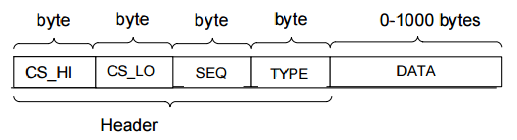
\includegraphics[width=1\linewidth]{Subpages/Billeder/Transportlag}
\caption{Transportlags protokol}
\label{fig:Transportlag}
\end{figure}

\textbf{CS\_HI:} Den mest betydende del af checksums-beregningen.\\
\textbf{CS\_LO:} Den mindst betydende del af checksums-beregningen.\\
\textbf{SEQ:} Sekvensnummer på den afsendte segment.\\
\textbf{TYPE:} 0 (DATA) 1 (ACK)\\
\textbf{DATA:} Payload på mellem 0-1000 bytes. Skal altid være af længden 0 ved ACK


\section{Send funktion}
I vores send funktion modtager vi parameterene "const char buf[]" og "short size". 

Vi starter med at tage den givne buffer, som indeholder vores data og lægger dataene over i en ny buffer, men nu reserverer vi de første 4 pladser i bufferen til vores header. 
Vi har defineret en ny konstant kaldet HDRSIZE, som er størrelsen på headeren. Dette er gjort for at der ikke bliver skabt forvirring omkring ACKSIZE, som i vores tilfælde et det samme som header størrelsen. 
Vi reserverer de første 4 pladser i bufferen med koden:
\begin{lstlisting}
for(int i = 0; i<size; i++)
{
	buffer[HDRSIZE+i] = buf[i];
}
\end{lstlisting}
I stedet for en for løkke kan man også bruge funktionen \textit{memcpy()}, som kopier et array over i et andet array.

Herefter lægger vi sekvensnummer og type på plads 2 og 3 i headeren. 
Vi beregner Checksummen ved hjælp af funktionen 
\begin{lstlisting}
checksum->calcChecksum(buffer, size+HDRSIZE);
\end{lstlisting}
Funktionen sørger både for at beregne checksummen, men også for at lægge den mest betydende del og mindst betydende del på henholdvis plads 0 og 1 i headeren.

Vi har lavet en do while løkke, som bliver kører så længe \textit{recieveAck er false}, hvilket betyder at vi ikke har modtaget den rigtige acknowledge. Løkken står for at sende bufferen videre til linklaget. 
For at vores send funktionen ikke skal stå og sende ubegænset har vi implementeret en counter, som tæller op hver gang vi modtager en forkert acknowledge. Når vi har fået 3 fejl i træk, breaker vi ud af løkken. 

Tilsidst sætter vi det gamle sekvensnummer til 2.

\section{Receive funktion}

Vi har implementeret vores receive funktionen ved at lave en while løkke, som tjekker om vores checksum og sekvensnummer er det rigtige. 
Checksum bliver lagt over i en variable kaldet receiveOk. 
For at kunne check summen og sekvensnummeret modtager vi en buffer linklaget. 
Dette gøres med funktionen: 
\begin{lstlisting}
n = link->receive(buffer,size+HDRSIZE);
\end{lstlisting}
Hvor n er størrelsen på bufferen vi modtager fra linklaget. Størrelsen bruges til at tjekket checksummen. 

Vi tester med en if løkke om vi modtager noget og hvis det er tilfældet tjekker vi om checksummen er korrekt. 

Efter vi har tjekket check checksummen sender vi en acknowledge, som enten fortæller at checksummen var korrekt eller at den var forkert. 

Vi tjekker yderlige at det gamle sekvensnummer \textit{old\_seqNo} er forskellige fra det nuværende sekevensnummer. Sekvensnummeret skifter fra 0 til 1 og tilbage hver gang en pakke er sendt. Derfor ved vi at hvis sekvensnumre ikke er forskellige får vi en forkert pakke.  

Vi har implementeret det med en if løkke. 
Er de to sekvensnumre er forskellige lægger vi den modtagende buffer og i en ny buffer, men nu uden headeren og returnerer størrelsen på den nye buffer.

Det gøres fordi at headeren kun er til for at tjekke om vores data er sendt korrekt.  
